\documentclass[12pt,a4paper]{report}

\usepackage{fontspec}
\usepackage{polyglossia}
\setmainlanguage{vietnamese}
\setmainfont{TeX Gyre Termes}
\usepackage{geometry}
\geometry{left=3cm,right=2cm,top=2.5cm,bottom=2.5cm}
\usepackage{graphicx}
\usepackage{float}
\usepackage{array}
\usepackage{booktabs}
\usepackage{longtable}
\usepackage{tabularx}
\usepackage{multirow}
\usepackage{xcolor}
\usepackage{hyperref}
\usepackage{tikz}
\usetikzlibrary{arrows.meta,positioning,fit}
\usepackage{caption}
\usepackage{subcaption}
\usepackage{enumitem}
\usepackage{titlesec}
\usepackage{fancyhdr}
\usepackage{setspace}
\usepackage{listings}

\hypersetup{
    colorlinks=true,
    linkcolor=black,
    citecolor=blue,
    urlcolor=blue
}

\onehalfspacing
\setlength{\parindent}{1.2cm}
\setlength{\parskip}{4pt}

\titleformat{\chapter}{\bfseries\Large}{Chương \thechapter.}{0.6em}{}
\titleformat{\section}{\bfseries\large}{\thesection}{0.6em}{}
\titleformat{\subsection}{\bfseries\normalsize}{\thesubsection}{0.6em}{}

\pagestyle{fancy}
\setlength{\headheight}{15pt}
\fancyhf{}
\lhead{Nhập môn An toàn thông tin}
\rhead{Cloud Security Demo}
\cfoot{\thepage}

\lstset{
    basicstyle=\ttfamily\small,
    breaklines=true,
    frame=single,
    columns=fullflexible
}

\begin{document}

\begin{titlepage}
    \centering
    {\bfseries\Large TRƯỜNG ĐẠI HỌC BÁCH KHOA HÀ NỘI\par}
    \vspace{0.3cm}
    {\bfseries\large VIỆN CÔNG NGHỆ THÔNG TIN VÀ TRUYỀN THÔNG\par}
    \vspace{2.2cm}
    {\bfseries\Large TIỂU LUẬN MÔN HỌC\par}
    \vspace{0.4cm}
    {\bfseries\Large NHẬP MÔN AN TOÀN THÔNG TIN\par}
    \vspace{1.8cm}
    {\bfseries\LARGE Điện toán đám mây và bảo mật điện toán đám mây\par}
    \vspace{0.4cm}
    {\Large Phân tích rủi ro, lỗ hổng và các cơ chế bảo vệ dữ liệu\par}
    \vspace{2cm}
    \begin{tabular}{ll}
        \textbf{Nhóm thực hiện:} & Đào Trường Anh - 20235639 \\
                                & Nguyễn Đồng Minh Anh - 20235646 \\
                                & Đoàn Đình Bằng - 20235662 \\
        \textbf{Giảng viên:}    & ...................................... \\
    \end{tabular}
    \vfill
    {\large Hà Nội, 2026\par}
\end{titlepage}

\pagenumbering{roman}
\tableofcontents
\listoffigures
\listoftables
\clearpage

\pagenumbering{arabic}

\chapter{Mở đầu}

\section{Lý do chọn đề tài}
Điện toán đám mây đã trở thành nền tảng quan trọng trong quá trình chuyển đổi số của doanh nghiệp, trường học và các tổ chức nhà nước. Thay vì đầu tư toàn bộ hạ tầng vật lý, tổ chức có thể thuê máy chủ, lưu trữ, cơ sở dữ liệu và dịch vụ bảo mật thông qua Internet. Mô hình này giúp triển khai nhanh, mở rộng linh hoạt và tối ưu chi phí vận hành.

Tuy nhiên, môi trường đám mây cũng tạo ra nhiều rủi ro an toàn thông tin. Dữ liệu có thể bị rò rỉ do bucket lưu trữ công khai, tài khoản bị cấp quyền quá mức, API thiếu kiểm soát, secret bị đặt trực tiếp trong cấu hình hoặc hệ thống thiếu giám sát. Các sự cố này thường không xuất phát từ lỗi của nhà cung cấp dịch vụ, mà đến từ việc người dùng cấu hình sai hoặc chưa hiểu rõ mô hình chia sẻ trách nhiệm.

Vì vậy, đề tài ``Điện toán đám mây và bảo mật điện toán đám mây'' được thực hiện nhằm hệ thống hóa kiến thức nền tảng, phân tích các rủi ro phổ biến và xây dựng một mô hình demo nhỏ để minh họa quá trình phát hiện và khắc phục lỗi bảo mật trong môi trường cloud.

\section{Mục tiêu nghiên cứu}
Đề tài hướng đến các mục tiêu chính sau:
\begin{itemize}
    \item Trình bày khái niệm, đặc trưng, mô hình dịch vụ và mô hình triển khai của điện toán đám mây.
    \item Phân tích các rủi ro an toàn thông tin thường gặp trên cloud, đặc biệt là rò rỉ dữ liệu, cấu hình sai, quản lý định danh yếu và lộ thông tin nhạy cảm.
    \item Trình bày các cơ chế bảo vệ như mã hóa, quản lý khóa, IAM, MFA, WAF, logging, monitoring và Zero Trust.
    \item Xây dựng case study với Flask, PostgreSQL, MinIO và Docker Compose để minh họa ba lỗi bảo mật: public storage bucket, IAM misconfiguration và credential leakage.
    \item Đề xuất khuyến nghị giúp vận hành hệ thống cloud an toàn hơn.
\end{itemize}

\section{Phạm vi nghiên cứu}
Báo cáo tập trung vào các nguyên lý và rủi ro phổ biến trong môi trường cloud ở mức nhập môn. Phần thực nghiệm sử dụng mô hình local bằng Docker để giả lập một hệ thống cloud nhỏ, gồm web application, cơ sở dữ liệu và object storage. Báo cáo không đi sâu vào triển khai production trên một nền tảng cụ thể như AWS, Microsoft Azure hoặc Google Cloud Platform.

\section{Phương pháp nghiên cứu}
Nhóm sử dụng bốn phương pháp chính:
\begin{itemize}
    \item \textbf{Nghiên cứu tài liệu:} tổng hợp kiến thức từ tài liệu chuẩn như NIST, CSA, ISO/IEC và OWASP.
    \item \textbf{Phân tích và tổng hợp:} phân loại các nguy cơ theo nhóm rủi ro và cơ chế phòng thủ tương ứng.
    \item \textbf{So sánh đánh giá:} đối chiếu trạng thái trước và sau khi áp dụng biện pháp bảo mật.
    \item \textbf{Nghiên cứu tình huống:} xây dựng demo để quan sát tác động của lỗi cấu hình và cách khắc phục.
\end{itemize}

\section{Bố cục báo cáo}
Báo cáo gồm bảy chương. Chương 1 giới thiệu đề tài. Chương 2 trình bày tổng quan điện toán đám mây. Chương 3 phân tích các nguy cơ an toàn thông tin. Chương 4 trình bày các cơ chế bảo mật. Chương 5 nói về quản lý rủi ro và tuân thủ. Chương 6 là case study thực nghiệm. Chương 7 tổng kết và nêu hướng phát triển.

\chapter{Tổng quan về điện toán đám mây}

\section{Khái niệm điện toán đám mây}
Điện toán đám mây là mô hình cung cấp tài nguyên công nghệ thông tin theo nhu cầu thông qua mạng Internet. Các tài nguyên này có thể bao gồm máy chủ, lưu trữ, cơ sở dữ liệu, mạng, nền tảng phát triển phần mềm và ứng dụng hoàn chỉnh. Người dùng không cần trực tiếp quản lý hạ tầng vật lý mà có thể thuê và sử dụng theo mức tiêu thụ thực tế.

Theo NIST, điện toán đám mây có năm đặc trưng cơ bản: tự phục vụ theo nhu cầu, truy cập rộng qua mạng, gộp tài nguyên, co giãn nhanh và đo lường dịch vụ. Các đặc trưng này giúp cloud trở thành nền tảng phù hợp cho hệ thống cần mở rộng nhanh, triển khai linh hoạt và tối ưu chi phí.

\section{Các mô hình dịch vụ}
\subsection{IaaS}
IaaS cung cấp hạ tầng như máy chủ ảo, ổ đĩa, mạng và firewall. Khách hàng kiểm soát hệ điều hành, ứng dụng và dữ liệu. Mô hình này linh hoạt nhưng yêu cầu người dùng có năng lực quản trị hệ thống.

\subsection{PaaS}
PaaS cung cấp môi trường chạy ứng dụng, middleware và công cụ phát triển. Nhà cung cấp quản lý phần lớn hạ tầng, còn người dùng tập trung vào mã nguồn và dữ liệu ứng dụng.

\subsection{SaaS}
SaaS cung cấp phần mềm hoàn chỉnh qua Internet. Người dùng chỉ sử dụng ứng dụng mà không cần quản trị hạ tầng hoặc nền tảng bên dưới.

\begin{table}[H]
\centering
\caption{So sánh các mô hình dịch vụ cloud}
\begin{tabularx}{\textwidth}{|X|X|X|X|}
\hline
\textbf{Tiêu chí} & \textbf{IaaS} & \textbf{PaaS} & \textbf{SaaS} \\
\hline
Mức kiểm soát & Cao & Trung bình & Thấp \\
\hline
Đối tượng chính & Quản trị hệ thống & Lập trình viên & Người dùng cuối \\
\hline
Khách hàng quản lý & OS, app, dữ liệu & App, dữ liệu & Cấu hình sử dụng \\
\hline
Ví dụ & VM, storage, network & App platform & Email, office suite \\
\hline
\end{tabularx}
\end{table}

\section{Các mô hình triển khai}
\textbf{Public Cloud} là mô hình cloud do nhà cung cấp bên thứ ba vận hành, nhiều khách hàng cùng sử dụng hạ tầng chung. \textbf{Private Cloud} phục vụ riêng một tổ chức, có mức kiểm soát cao hơn nhưng chi phí lớn hơn. \textbf{Hybrid Cloud} kết hợp public và private cloud. \textbf{Multi-Cloud} sử dụng nhiều nhà cung cấp cloud để giảm phụ thuộc và tăng tính linh hoạt.

\section{Shared Responsibility Model}
Mô hình chia sẻ trách nhiệm là nguyên tắc quan trọng trong bảo mật cloud. Nhà cung cấp chịu trách nhiệm bảo vệ hạ tầng bên dưới, còn khách hàng chịu trách nhiệm bảo vệ dữ liệu, tài khoản, cấu hình dịch vụ và ứng dụng của mình. Rất nhiều sự cố cloud xảy ra khi khách hàng hiểu sai ranh giới trách nhiệm này.

\section{Vai trò của cloud trong doanh nghiệp}
Cloud giúp doanh nghiệp triển khai sản phẩm nhanh hơn, mở rộng hệ thống theo lưu lượng thực tế, tối ưu chi phí ban đầu và tiếp cận các dịch vụ bảo mật hiện đại. Tuy nhiên, lợi ích này chỉ đạt được khi hệ thống được thiết kế và vận hành với tư duy bảo mật ngay từ đầu.

\chapter{Các nguy cơ an toàn thông tin trên điện toán đám mây}

\section{Mô hình CIA}
Ba mục tiêu cơ bản của an toàn thông tin là bảo mật, toàn vẹn và sẵn sàng. Trong môi trường cloud, dữ liệu cần được bảo vệ khỏi truy cập trái phép, không bị thay đổi ngoài ý muốn và luôn sẵn sàng khi người dùng hợp lệ cần sử dụng.

\section{Rò rỉ dữ liệu}
Rò rỉ dữ liệu có thể xảy ra khi dữ liệu nhạy cảm được lưu trong bucket công khai, database mở cổng ra Internet, secret bị commit lên repository hoặc API trả về quá nhiều thông tin. Đây là một trong những rủi ro nghiêm trọng nhất vì ảnh hưởng trực tiếp đến khách hàng, uy tín và trách nhiệm pháp lý của tổ chức.

\section{Cấu hình sai}
Cấu hình sai là nguyên nhân phổ biến của sự cố cloud. Ví dụ: object storage public, security group mở toàn bộ cổng, IAM policy cấp quyền quá rộng, logging bị tắt hoặc khóa mã hóa không được xoay vòng. Điểm nguy hiểm là lỗi cấu hình thường rất nhỏ nhưng có thể tạo ra hậu quả lớn.

\section{API không an toàn}
Cloud service và web application thường giao tiếp qua API. Nếu API thiếu xác thực, thiếu phân quyền, không kiểm tra input hoặc không giới hạn tốc độ, attacker có thể khai thác để đọc dữ liệu, sửa dữ liệu hoặc gây quá tải hệ thống.

\section{Quản lý định danh yếu kém}
Tài khoản cloud thường có quyền truy cập nhiều tài nguyên quan trọng. Nếu không bật MFA, dùng mật khẩu yếu hoặc cấp quyền vượt nhu cầu, attacker có thể chiếm tài khoản và mở rộng quyền truy cập trong hệ thống.

\section{Mối đe dọa nội bộ}
Insider threat đến từ nhân viên, nhà thầu hoặc tài khoản nội bộ bị chiếm quyền. Trong cloud, insider có thể sao chép dữ liệu, thay đổi cấu hình, xóa log hoặc tạo backdoor nếu quyền truy cập không được giới hạn và giám sát.

\section{Lỗ hổng công nghệ dùng chung}
Cloud dựa trên ảo hóa, container, hypervisor và hạ tầng dùng chung. Nếu có lỗi ở lớp nền tảng hoặc cấu hình cô lập tenant không đúng, rủi ro có thể lan rộng giữa các môi trường khác nhau.

\section{Tấn công từ chối dịch vụ}
DDoS làm cạn tài nguyên mạng, CPU, memory hoặc quota dịch vụ. Dù cloud có khả năng mở rộng, hệ thống vẫn cần rate limiting, autoscaling hợp lý, CDN, WAF và cơ chế cảnh báo để giảm tác động.

\chapter{Các cơ chế bảo mật trên Cloud}

\section{Bảo vệ dữ liệu bằng mật mã học}
Dữ liệu cần được mã hóa khi lưu trữ và khi truyền tải. Mã hóa dữ liệu lưu trữ giúp giảm thiểu tác động nếu thiết bị lưu trữ hoặc bản sao dữ liệu bị truy cập trái phép. Mã hóa dữ liệu truyền tải, thường thông qua TLS, giúp bảo vệ dữ liệu khỏi nghe lén và chỉnh sửa trên đường truyền.

\section{Quản lý khóa và chứng thư số}
Mã hóa chỉ hiệu quả khi khóa được quản lý an toàn. KMS hỗ trợ tạo, lưu trữ, phân quyền và xoay vòng khóa. HSM cung cấp môi trường phần cứng an toàn hơn cho khóa quan trọng. PKI và Certificate Authority giúp xác thực danh tính dịch vụ và thiết lập kết nối tin cậy.

\section{Quản lý định danh và kiểm soát truy cập}
IAM là lớp bảo vệ trung tâm trong cloud. Các nguyên tắc quan trọng gồm:
\begin{itemize}
    \item bật MFA cho tài khoản quan trọng;
    \item áp dụng least privilege;
    \item phân quyền theo vai trò bằng RBAC;
    \item tách tài khoản quản trị và tài khoản sử dụng thường ngày;
    \item định kỳ rà soát quyền truy cập.
\end{itemize}

\section{Bảo mật mạng và ứng dụng}
Bảo mật mạng cloud bao gồm phân vùng mạng, firewall, security group, private subnet và kiểm soát truy cập vào dịch vụ nội bộ. Với web application, WAF giúp phát hiện và chặn các mẫu tấn công phổ biến như SQL Injection, XSS, path traversal hoặc request bất thường.

\section{Giám sát và ứng phó sự cố}
Logging và audit trail giúp truy vết hành vi người dùng và dịch vụ. IDS/IPS, SIEM và hệ thống cảnh báo giúp phát hiện sự kiện bất thường. Quy trình incident response giúp tổ chức phản ứng có thứ tự khi xảy ra sự cố, bao gồm phát hiện, cô lập, xử lý, khôi phục và rút kinh nghiệm.

\section{Các mô hình bảo mật hiện đại}
Zero Trust đặt giả định rằng không có thành phần nào mặc nhiên đáng tin cậy. Mọi request đều cần được xác thực, phân quyền và đánh giá ngữ cảnh. Defense in Depth triển khai nhiều lớp bảo vệ để khi một lớp thất bại, các lớp khác vẫn giảm thiểu tác động. Security by Design yêu cầu bảo mật được đưa vào từ giai đoạn thiết kế, không chỉ bổ sung sau khi hệ thống đã hoàn thành.

\chapter{Quản lý rủi ro và tuân thủ trong điện toán đám mây}

\section{Quy trình quản lý rủi ro}
Quản lý rủi ro bắt đầu bằng việc xác định tài sản cần bảo vệ, chẳng hạn dữ liệu khách hàng, tài khoản quản trị, khóa truy cập, database và log hệ thống. Sau đó, nhóm cần xác định mối đe dọa, đánh giá khả năng xảy ra và mức độ tác động, rồi lựa chọn biện pháp giảm thiểu phù hợp.

\begin{table}[H]
\centering
\caption{Ví dụ ma trận đánh giá rủi ro}
\begin{tabularx}{\textwidth}{|X|c|c|X|}
\hline
\textbf{Rủi ro} & \textbf{Khả năng} & \textbf{Tác động} & \textbf{Biện pháp giảm thiểu} \\
\hline
Bucket public làm lộ dữ liệu & Cao & Cao & Private bucket, signed URL, audit policy \\
\hline
User thường có quyền admin & Trung bình & Cao & RBAC, least privilege, review quyền \\
\hline
Secret nằm trong cấu hình rõ & Cao & Cao & Secret manager, mã hóa, tách khỏi source code \\
\hline
\end{tabularx}
\end{table}

\section{Các tiêu chuẩn và khung tham chiếu}
Một số khung tham chiếu thường dùng trong bảo mật cloud gồm NIST Cybersecurity Framework, CSA Cloud Controls Matrix, ISO/IEC 27001, ISO/IEC 27017 và ISO/IEC 27018. Các tài liệu này giúp tổ chức xây dựng chính sách, kiểm soát rủi ro và chứng minh mức độ tuân thủ.

\section{Bảo vệ dữ liệu cá nhân và yêu cầu pháp lý}
Dữ liệu cá nhân cần được xử lý theo nguyên tắc tối thiểu hóa, có mục đích rõ ràng, được bảo vệ bằng biện pháp kỹ thuật phù hợp và có khả năng truy vết. Khi xảy ra rò rỉ dữ liệu, tổ chức có thể phải thông báo sự cố, khắc phục hậu quả và chịu trách nhiệm pháp lý.

\section{Các chỉ số đánh giá hiệu quả bảo mật}
Một số chỉ số có thể dùng để đánh giá hiệu quả bảo mật:
\begin{itemize}
    \item \textbf{MTTD:} thời gian trung bình để phát hiện sự cố.
    \item \textbf{MTTR:} thời gian trung bình để phản ứng hoặc khôi phục.
    \item \textbf{MFA Adoption Rate:} tỷ lệ tài khoản đã bật MFA.
    \item \textbf{Encryption Coverage Rate:} tỷ lệ dữ liệu đã được mã hóa.
\end{itemize}

\chapter{Nghiên cứu tình huống: Cloud Security Demo}

\section{Mô tả bài toán}
Nhóm xây dựng một hệ thống demo nhỏ để mô phỏng các lỗi bảo mật thường gặp trong môi trường cloud. Hệ thống gồm web application viết bằng Flask, cơ sở dữ liệu PostgreSQL và dịch vụ object storage MinIO. Toàn bộ môi trường chạy bằng Docker Compose để dễ triển khai, tái hiện và trình bày.

Mục tiêu của case study là minh họa ba rủi ro chính:
\begin{itemize}
    \item \textbf{Public Storage Bucket:} bucket lưu trữ dữ liệu khách hàng bị cấu hình công khai.
    \item \textbf{IAM Misconfiguration:} tài khoản người dùng thường bị cấp nhầm quyền quản trị.
    \item \textbf{Credential Leakage:} secret và credential được đặt trực tiếp trong cấu hình ở dạng rõ.
\end{itemize}

\section{Kiến trúc hệ thống đề xuất}
\begin{figure}[H]
\centering
\resizebox{\textwidth}{!}{%
\begin{tikzpicture}[
    node distance=1.6cm,
    box/.style={draw, rounded corners, minimum width=3.3cm, minimum height=1.1cm, align=center, fill=blue!5},
    risk/.style={draw=red!70, rounded corners, minimum width=3.3cm, minimum height=1.1cm, align=center, fill=red!5},
    secure/.style={draw=green!60!black, rounded corners, minimum width=3.3cm, minimum height=1.1cm, align=center, fill=green!5},
    arrow/.style={-Latex, thick}
]
\node[box] (user) {Người dùng\\Trình duyệt};
\node[risk, below=of user] (attacker) {Attacker\\Truy cập object public};
\node[box, right=3.2cm of user] (web) {Flask Web App\\localhost:5000};
\node[box, right=3.2cm of web, yshift=1.2cm] (db) {PostgreSQL\\Dữ liệu khách hàng};
\node[risk, right=3.2cm of web, yshift=-1.2cm] (minio) {MinIO Object Storage\\public-customer-data};
\node[secure, below=1.4cm of web] (secret) {Secret Protection\\Encrypted secret};
\draw[arrow] (user) -- node[above]{HTTP} (web);
\draw[arrow] (web) -- node[above]{SQL} (db);
\draw[arrow] (web) -- node[below]{S3 API} (minio);
\draw[arrow] (attacker) -- node[below]{public URL} (minio);
\draw[arrow] (secret) -- (web);
\node[draw, dashed, rounded corners, fit=(web)(db)(minio)(secret), inner sep=0.45cm, label=above:Docker network \texttt{cloud-lab}] {};
\end{tikzpicture}
}
\caption{Kiến trúc hệ thống Cloud Security Demo}
\label{fig:architecture}
\end{figure}

Các thành phần chính gồm:
\begin{itemize}
    \item \textbf{Flask Web App:} cung cấp giao diện đăng nhập, xem dữ liệu khách hàng, truy cập storage, trang admin và trang minh họa rủi ro cấu hình.
    \item \textbf{PostgreSQL:} lưu dữ liệu khách hàng và audit log mẫu.
    \item \textbf{MinIO:} giả lập dịch vụ object storage tương tự Amazon S3.
    \item \textbf{Docker Compose:} khởi chạy toàn bộ môi trường thực nghiệm.
\end{itemize}

\begin{figure}[H]
    \centering
    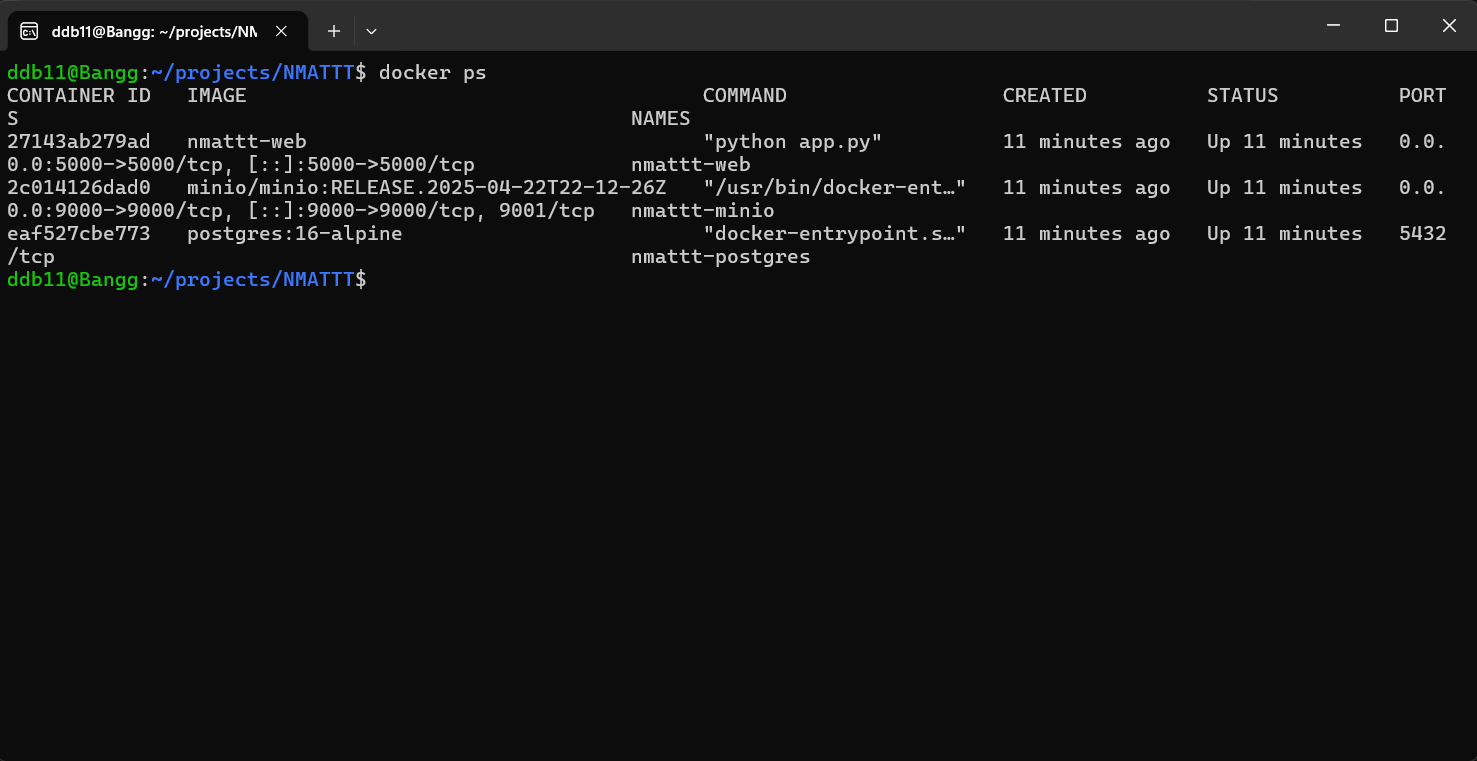
\includegraphics[width=0.92\textwidth]{../pictures/02-docker-compose-ps.png}
    \caption{Các container của môi trường demo đang hoạt động}
    \label{fig:docker-ps}
\end{figure}

\section{Tài sản cần bảo vệ}
Trong mô hình demo, tài sản quan trọng gồm dữ liệu khách hàng trong PostgreSQL, file dữ liệu trong bucket MinIO, tài khoản quản trị, thông tin truy cập database và access key của MinIO.

\begin{figure}[H]
    \centering
    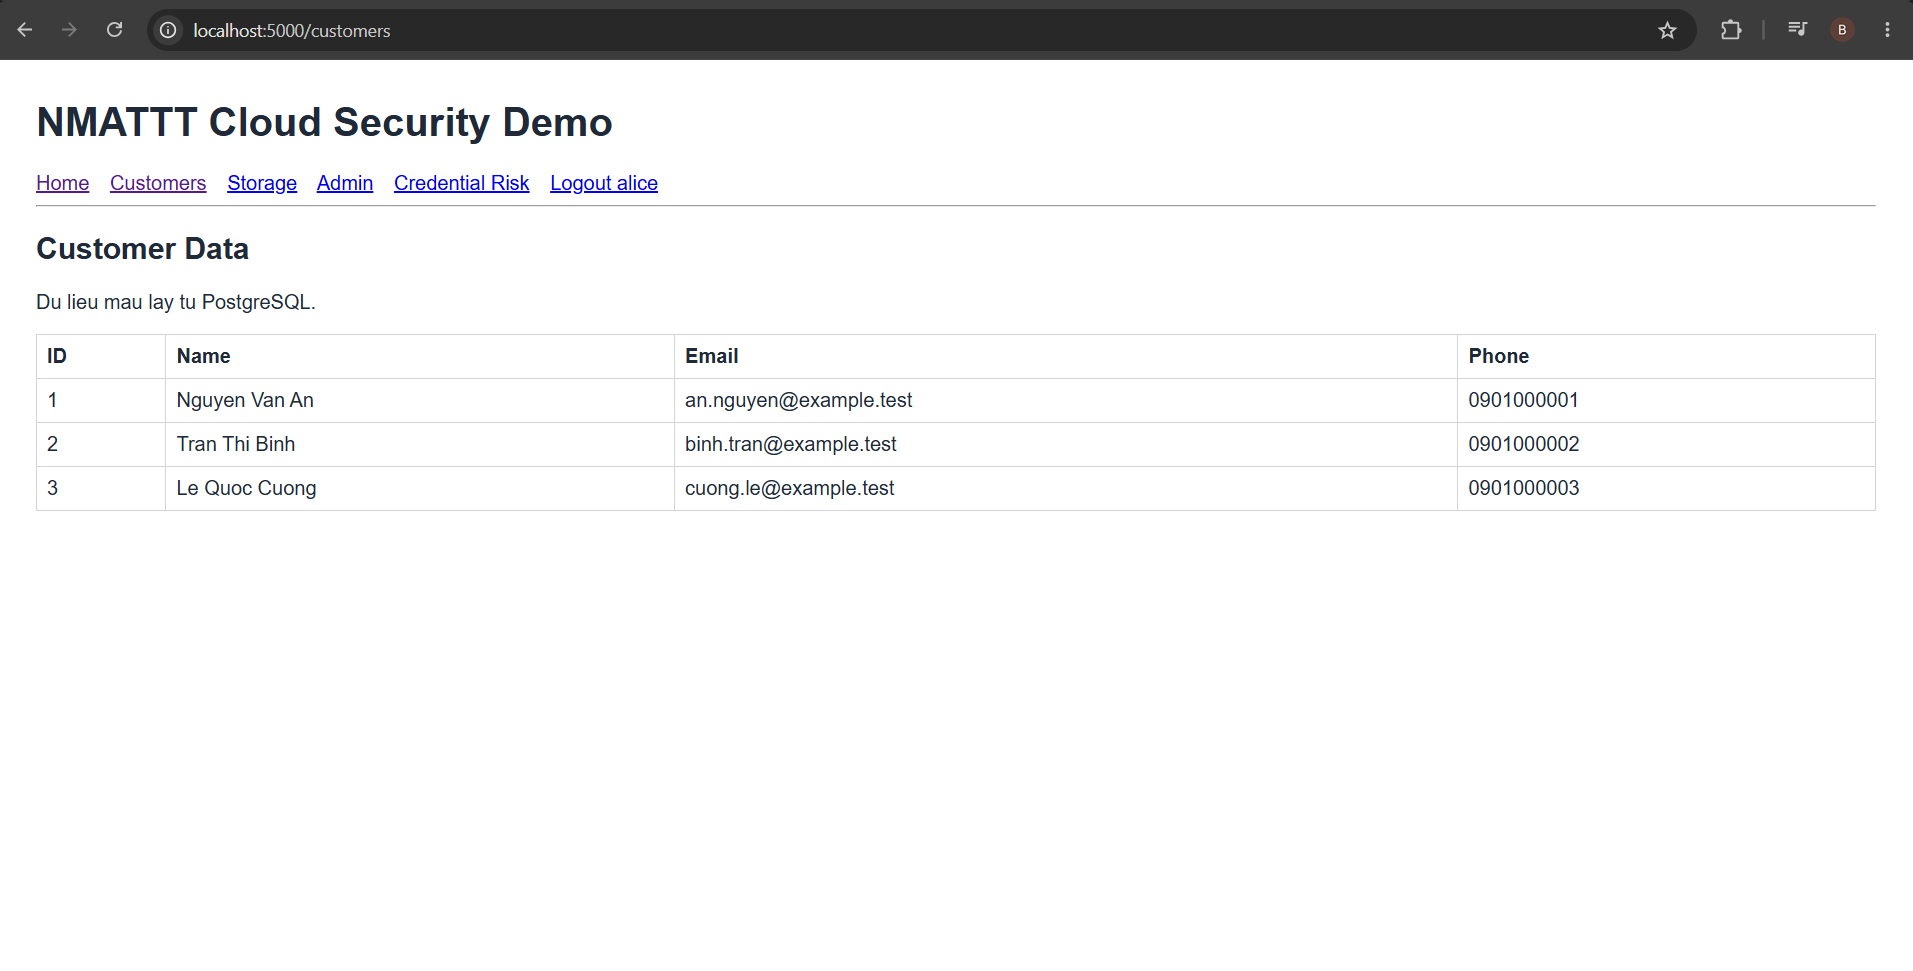
\includegraphics[width=0.92\textwidth]{../pictures/05-customers-postgresql.png}
    \caption{Dữ liệu khách hàng được đọc từ PostgreSQL}
    \label{fig:customers}
\end{figure}

\begin{figure}[H]
    \centering
    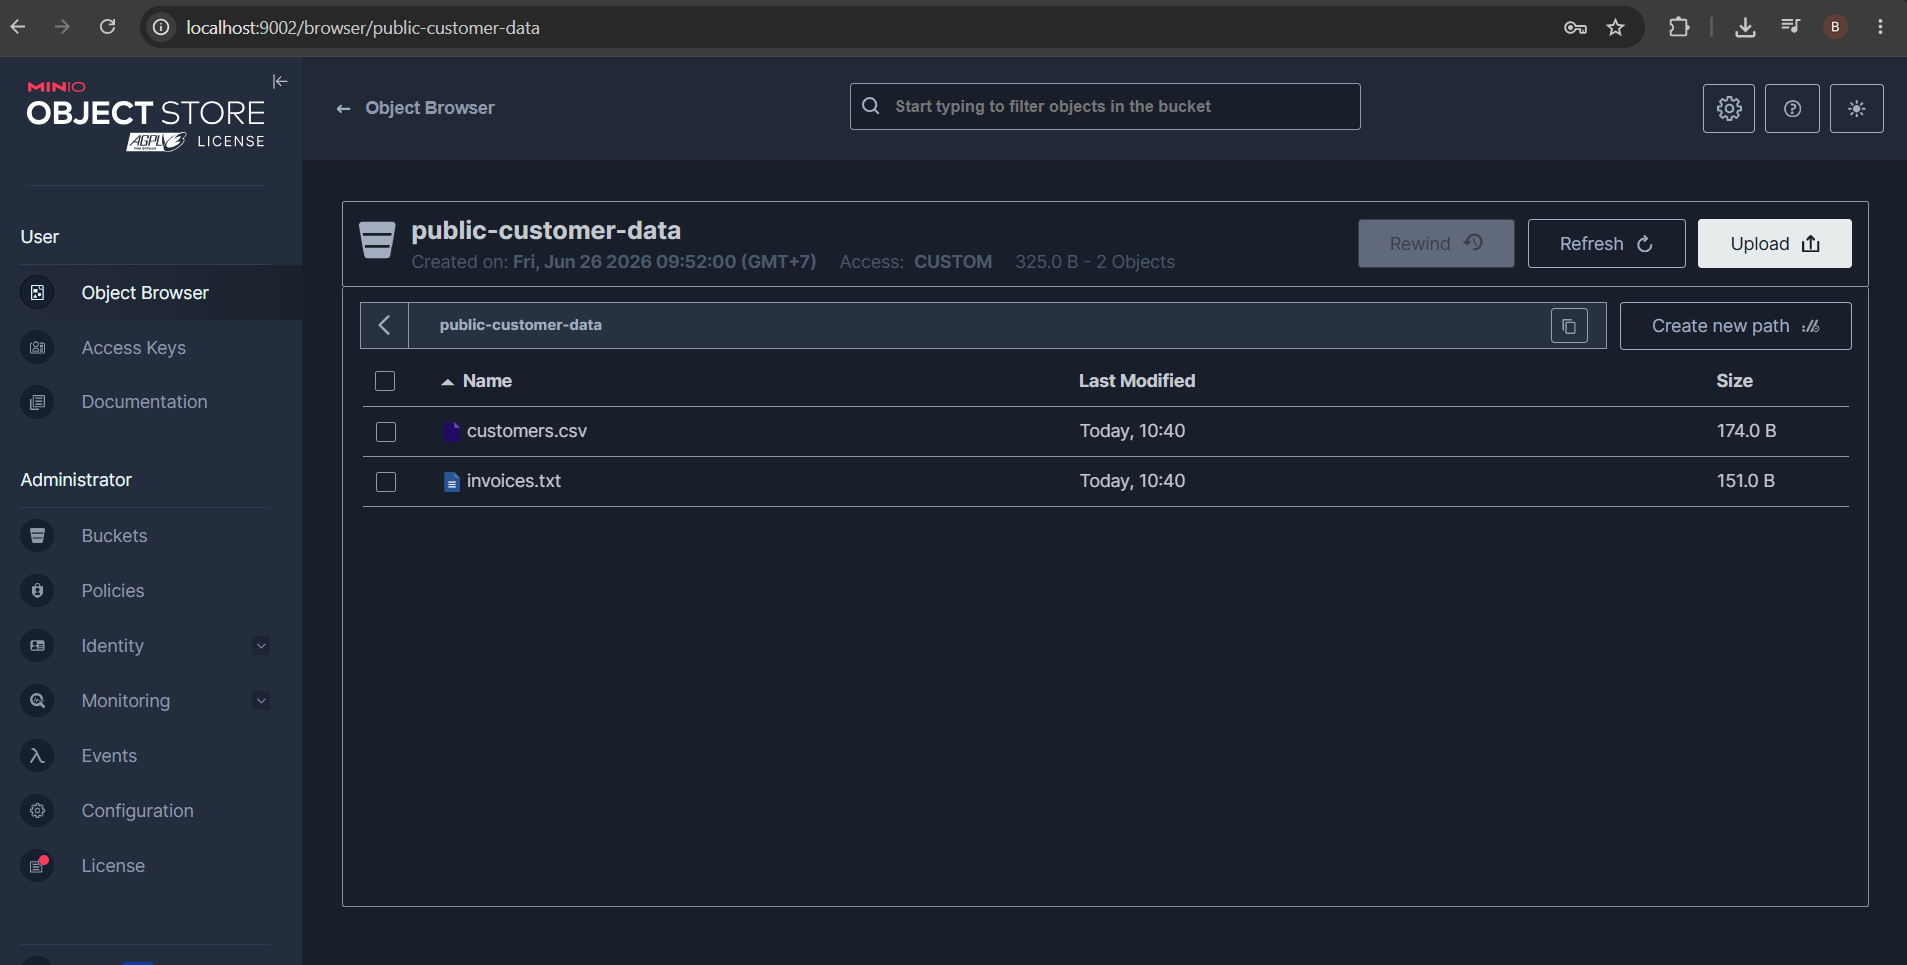
\includegraphics[width=0.92\textwidth]{../pictures/10-minio-console-public-bucket.png}
    \caption{Bucket \texttt{public-customer-data} trên MinIO Console}
    \label{fig:minio-console}
\end{figure}

\section{Phân tích mối đe dọa theo STRIDE}
\begin{longtable}{|p{2.8cm}|p{4.6cm}|p{5.8cm}|}
\caption{Phân tích mối đe dọa theo STRIDE trong case study}
\label{tab:stride}\\
\hline
\textbf{Nhóm STRIDE} & \textbf{Mối đe dọa} & \textbf{Biện pháp giảm thiểu} \\
\hline
\endfirsthead
\hline
\textbf{Nhóm STRIDE} & \textbf{Mối đe dọa} & \textbf{Biện pháp giảm thiểu} \\
\hline
\endhead
Spoofing & Attacker sử dụng tài khoản yếu hoặc credential bị lộ để đăng nhập. & MFA, mật khẩu mạnh, giới hạn đăng nhập, tách tài khoản admin. \\
\hline
Tampering & Dữ liệu trong bucket hoặc database bị thay đổi trái phép. & Phân quyền ghi, checksum, audit log, versioning. \\
\hline
Repudiation & Người dùng phủ nhận hành động do thiếu log. & Audit trail, ghi log truy cập, đồng bộ thời gian. \\
\hline
Information Disclosure & Bucket public hoặc secret plaintext làm lộ dữ liệu. & Private bucket, signed URL, mã hóa secret, không commit credential. \\
\hline
Denial of Service & Request bất thường gây quá tải web app hoặc storage. & Rate limiting, WAF, giám sát tài nguyên, cảnh báo. \\
\hline
Elevation of Privilege & User thường truy cập được trang admin. & RBAC, least privilege, kiểm tra quyền ở server side. \\
\hline
\end{longtable}

\section{Kịch bản 1: Public Storage Bucket}
Ở chế độ vulnerable, web app hiển thị đường dẫn đến object trong bucket. Do bucket được cấu hình công khai, người dùng có thể mở trực tiếp file dữ liệu mà không cần xác thực.

\begin{figure}[H]
    \centering
    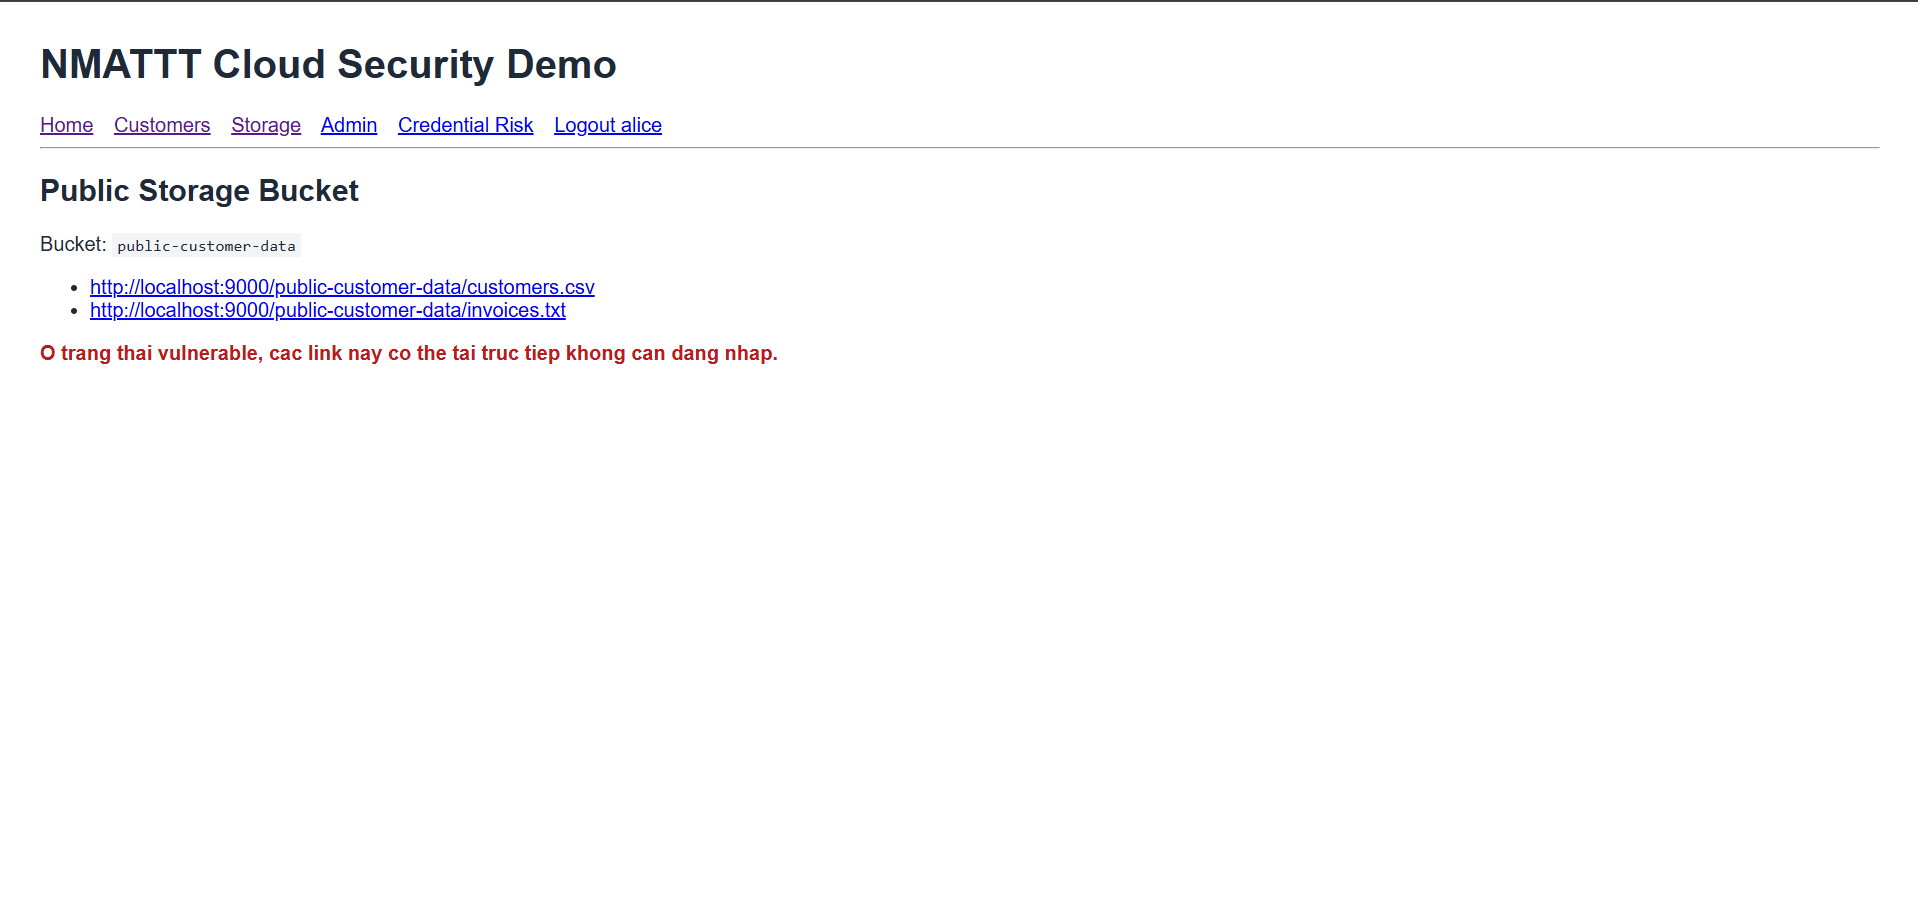
\includegraphics[width=0.92\textwidth]{../pictures/06-storage-public-bucket.png}
    \caption{Bucket công khai trong chế độ vulnerable}
    \label{fig:public-bucket}
\end{figure}

\begin{figure}[H]
    \centering
    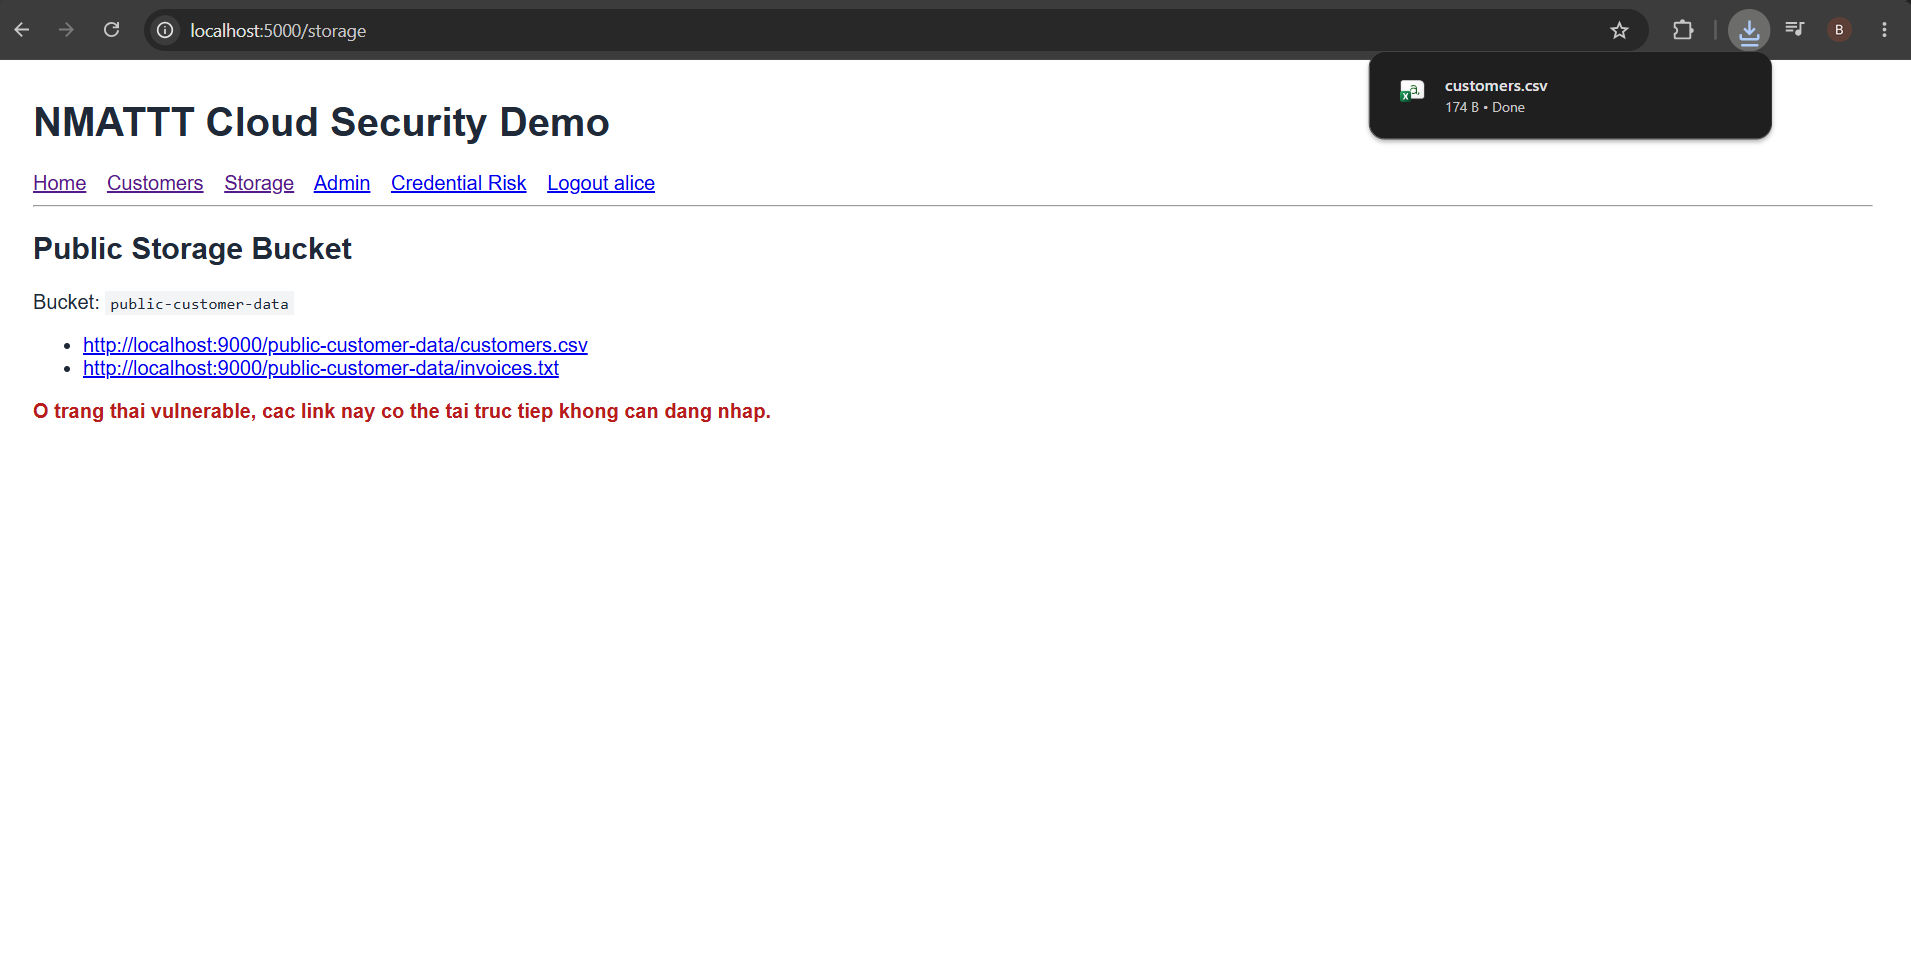
\includegraphics[width=0.92\textwidth]{../pictures/07-public-object-customers-csv.png}
    \caption{Truy cập trực tiếp object \texttt{customers.csv} không cần xác thực}
    \label{fig:public-object}
\end{figure}

\section{Kịch bản 2: IAM Misconfiguration}
Tài khoản \texttt{alice} là người dùng thường, nhưng ở chế độ vulnerable tài khoản này vẫn truy cập được trang \texttt{/admin}. Đây là ví dụ điển hình của lỗi phân quyền server side.

\begin{figure}[H]
    \centering
    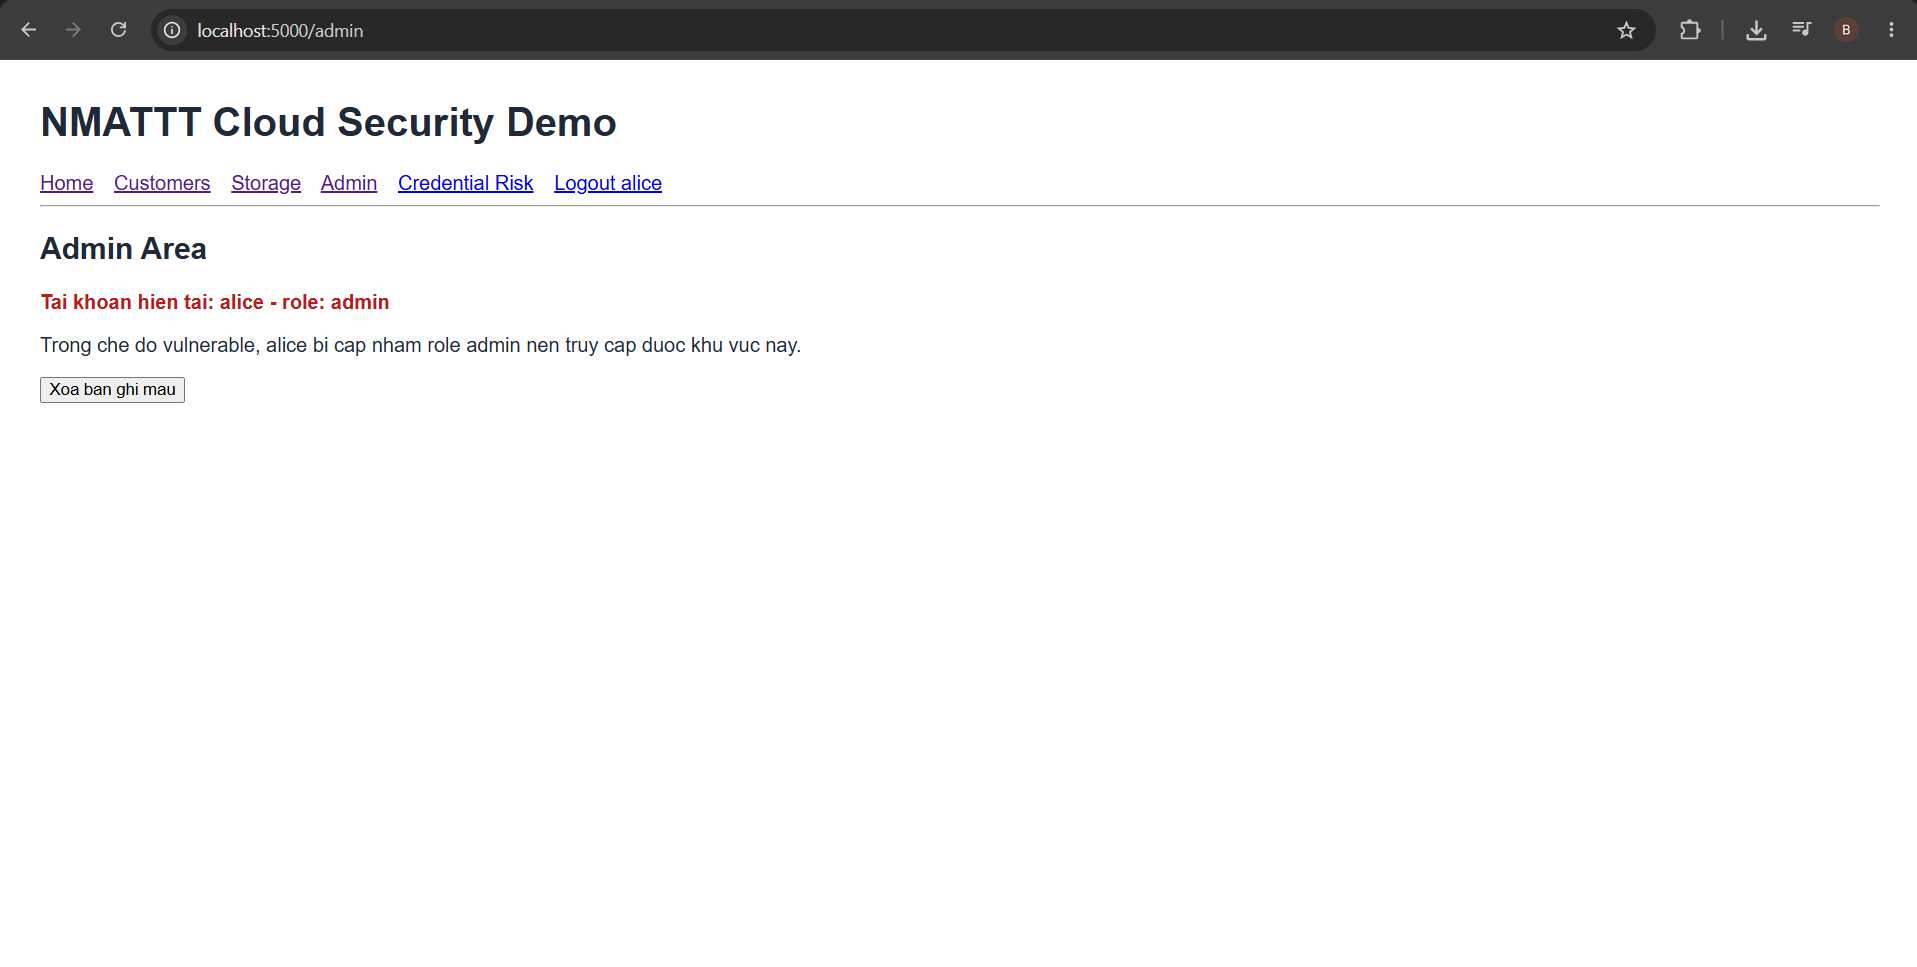
\includegraphics[width=0.92\textwidth]{../pictures/08-admin-vulnerable-alice.png}
    \caption{Tài khoản \texttt{alice} truy cập được trang admin trong chế độ vulnerable}
    \label{fig:iam-vulnerable}
\end{figure}

\section{Kịch bản 3: Credential Leakage}
Ở chế độ plaintext, thông tin nhạy cảm như mật khẩu database và MinIO secret key xuất hiện trong cấu hình. Nếu repository hoặc file cấu hình bị lộ, attacker có thể dùng các secret này để truy cập dịch vụ nội bộ.

\begin{figure}[H]
    \centering
    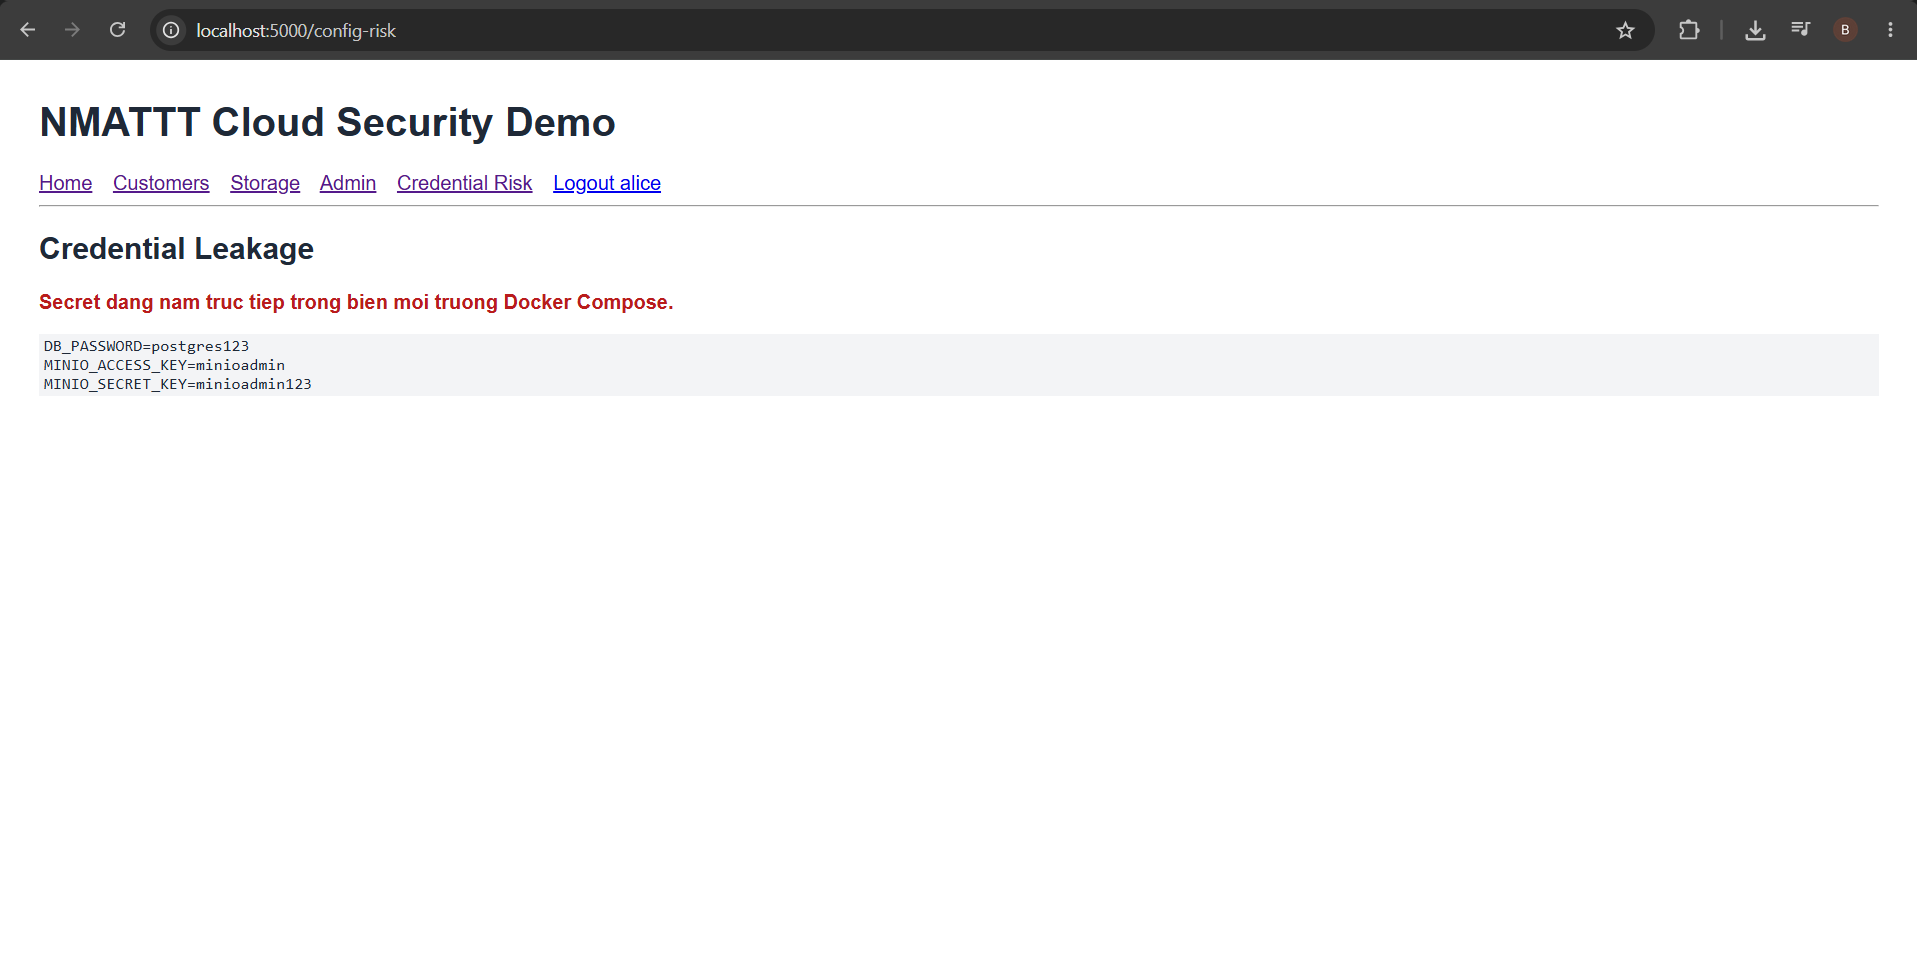
\includegraphics[width=0.92\textwidth]{../pictures/09-config-risk-plaintext.png}
    \caption{Credential được hiển thị ở dạng rõ trong chế độ vulnerable}
    \label{fig:plaintext-secret}
\end{figure}

\begin{figure}[H]
    \centering
    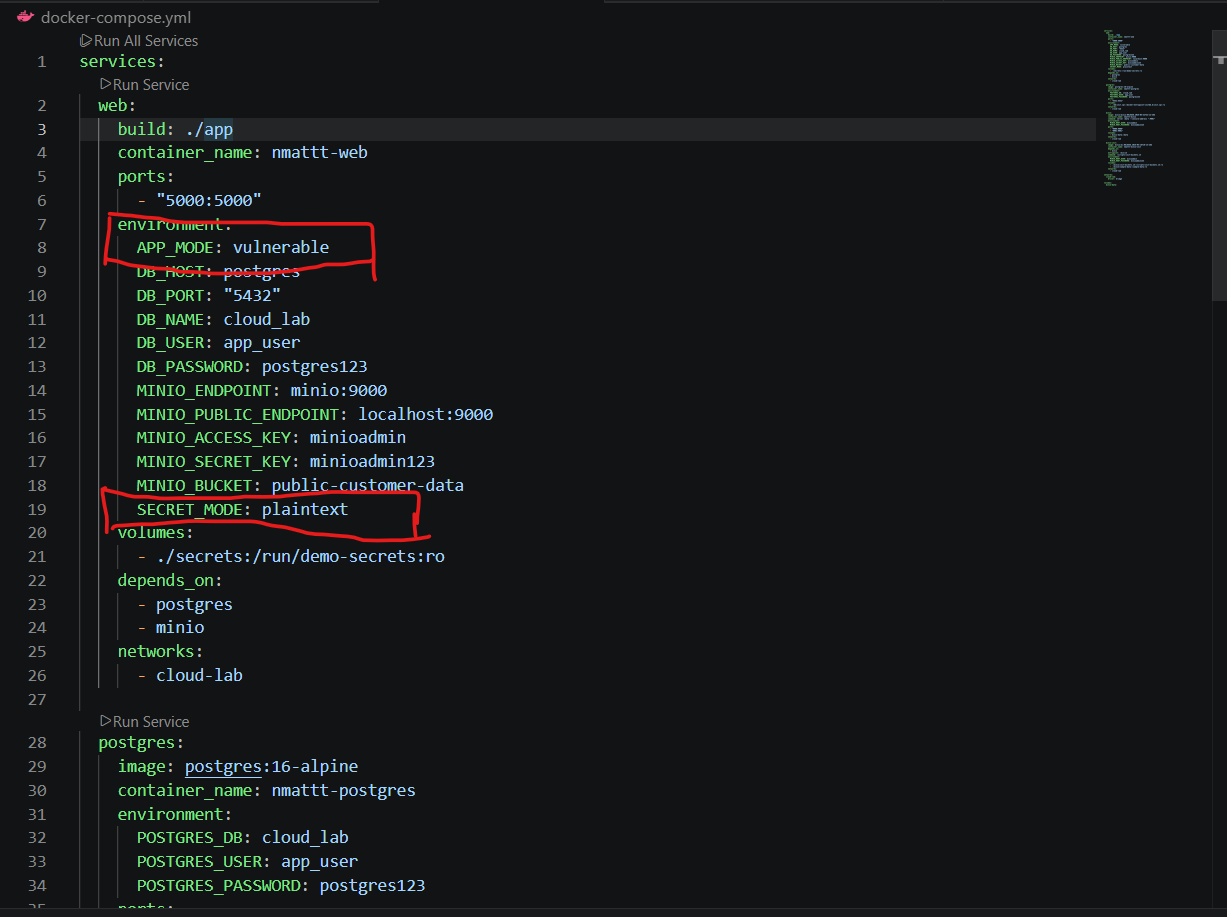
\includegraphics[width=0.82\textwidth]{../pictures/11-1-before.png}
    \caption{Cấu hình trước khi khắc phục: \texttt{APP\_MODE=vulnerable}, \texttt{SECRET\_MODE=plaintext}}
    \label{fig:before-config}
\end{figure}

\section{Biện pháp khắc phục}
Nhóm chuyển hệ thống sang chế độ fixed. Các thay đổi chính gồm:
\begin{itemize}
    \item chuyển bucket từ public sang private;
    \item kiểm tra quyền truy cập trang admin theo vai trò;
    \item tách secret khỏi mã nguồn và lưu dưới dạng mã hóa;
    \item chỉ giải mã secret trong runtime khi ứng dụng cần sử dụng.
\end{itemize}

\begin{figure}[H]
    \centering
    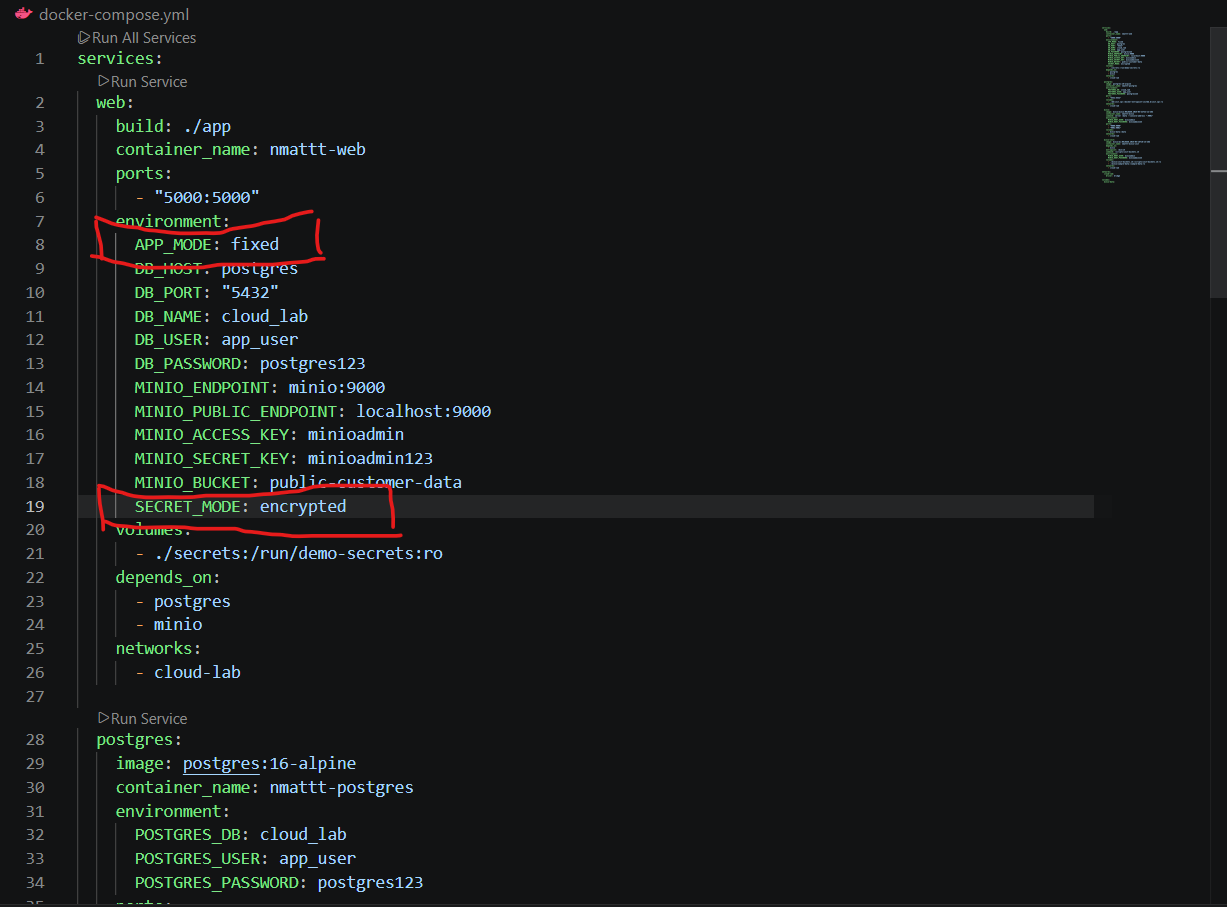
\includegraphics[width=0.82\textwidth]{../pictures/11-2-after.png}
    \caption{Cấu hình sau khi khắc phục: \texttt{APP\_MODE=fixed}, \texttt{SECRET\_MODE=encrypted}}
    \label{fig:after-config}
\end{figure}

\begin{figure}[H]
    \centering
    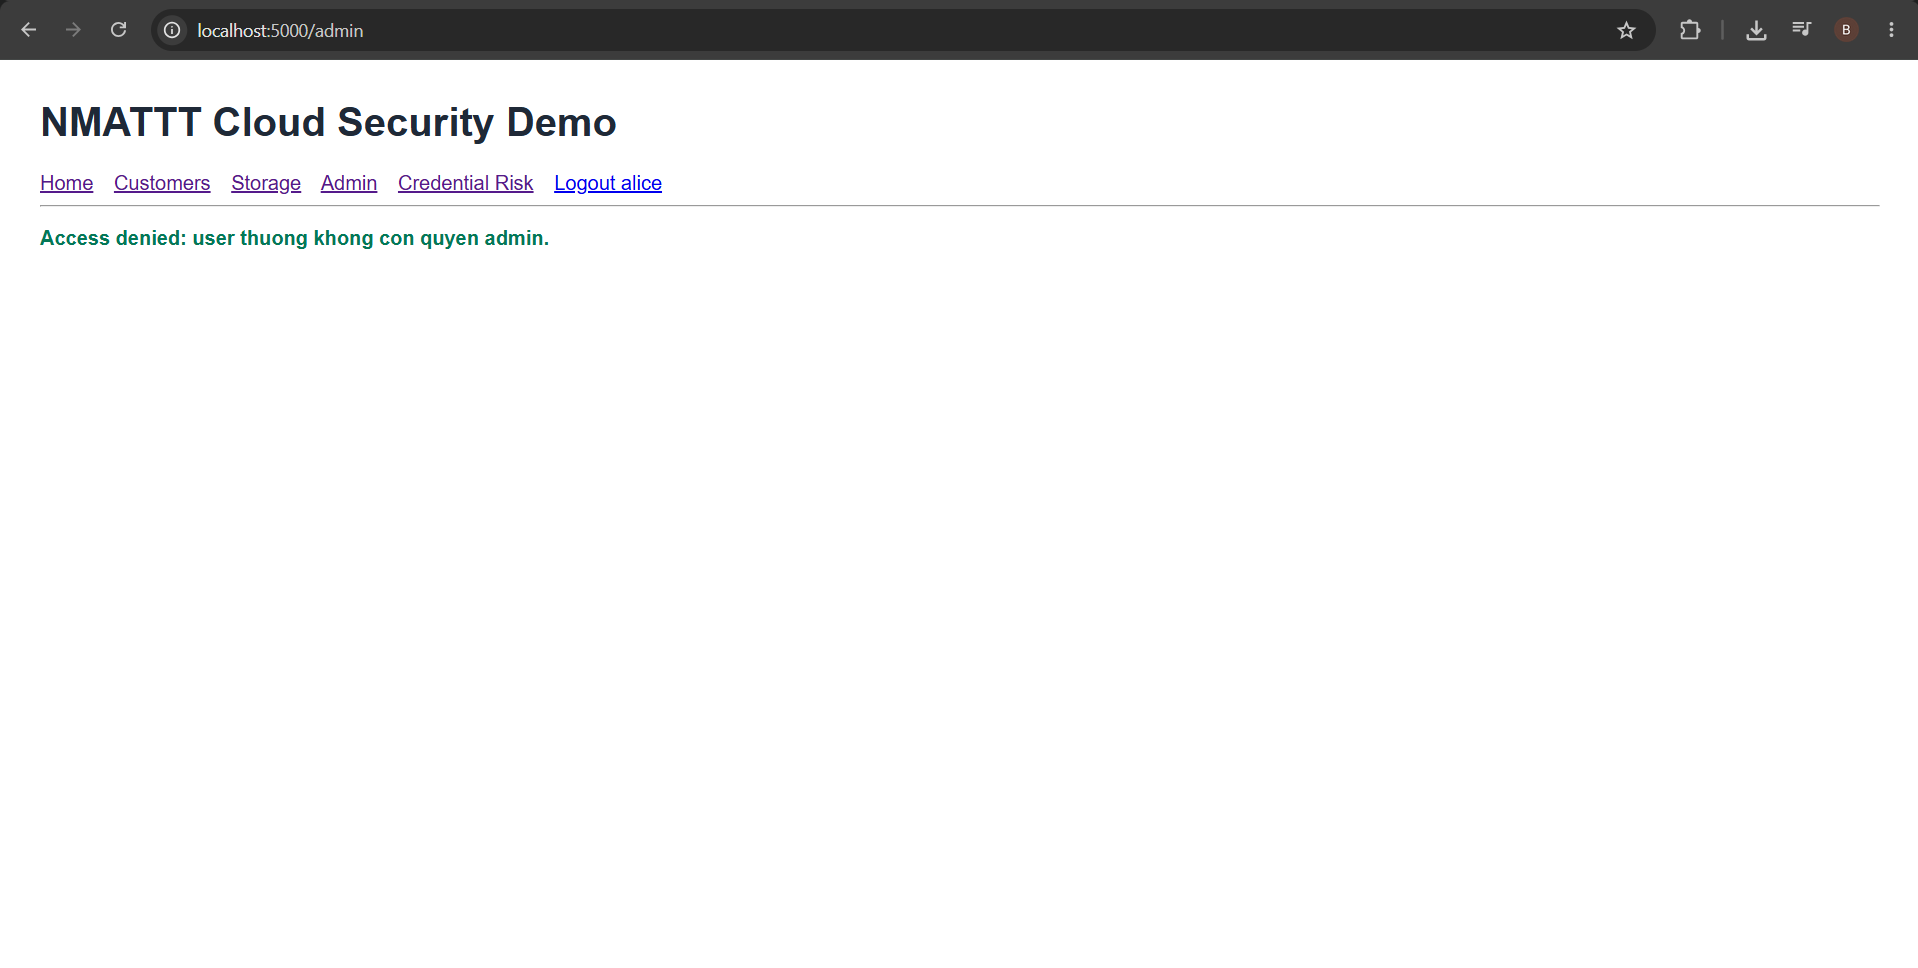
\includegraphics[width=0.92\textwidth]{../pictures/11-admin-fixed-alice-denied.png}
    \caption{Tài khoản \texttt{alice} bị chặn khỏi trang admin sau khi khắc phục}
    \label{fig:admin-denied}
\end{figure}

\begin{figure}[H]
    \centering
    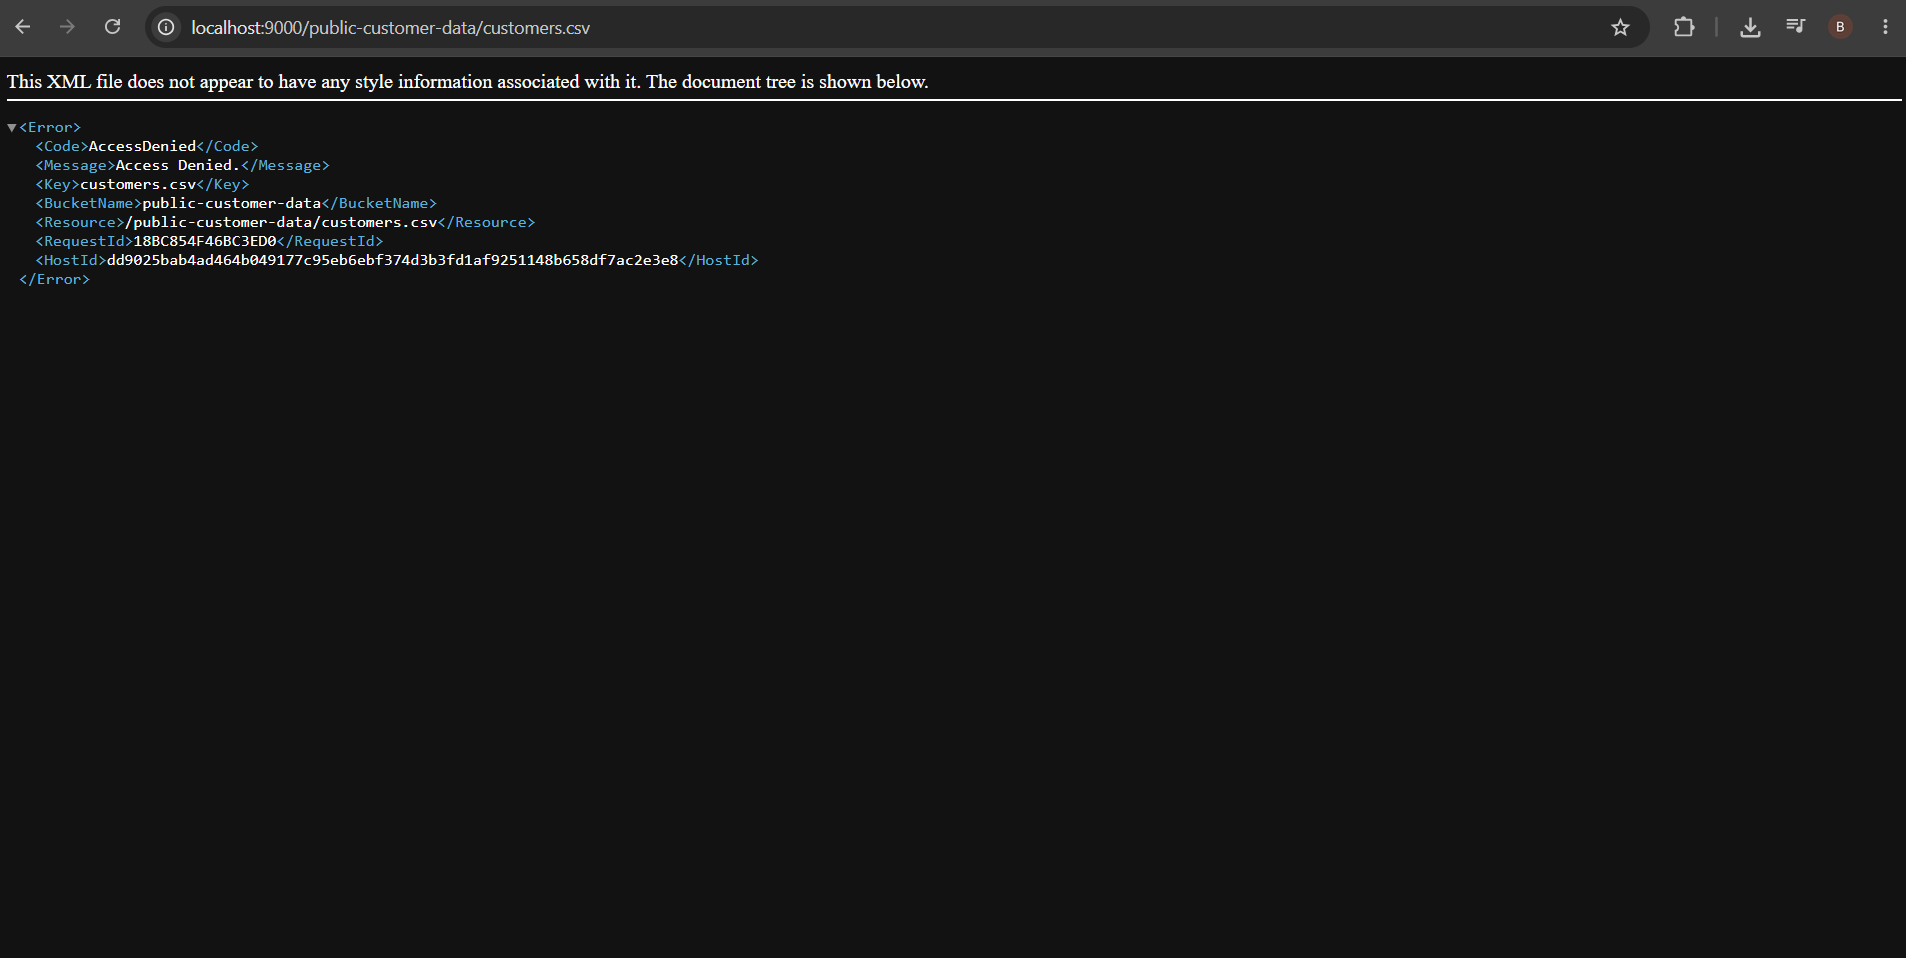
\includegraphics[width=0.92\textwidth]{../pictures/13-public-object-denied-fixed.png}
    \caption{Truy cập trực tiếp object bị từ chối sau khi bucket chuyển sang private}
    \label{fig:object-denied}
\end{figure}

\begin{figure}[H]
    \centering
    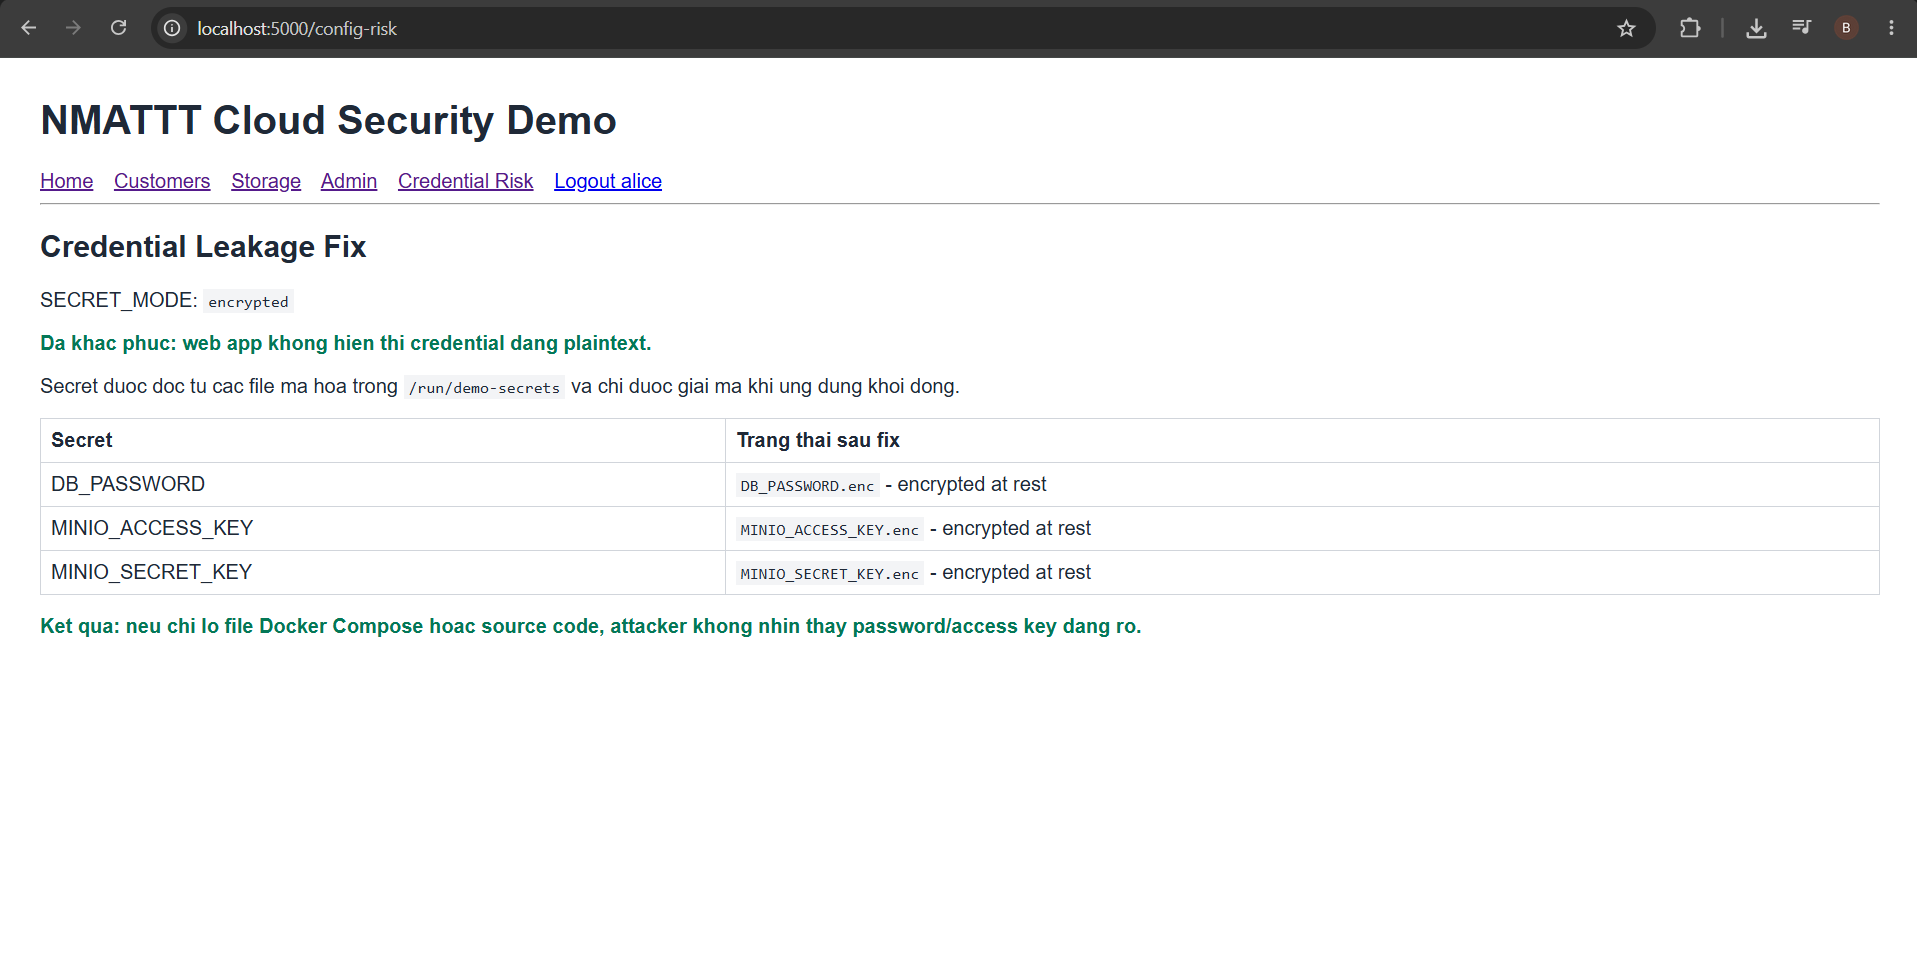
\includegraphics[width=0.92\textwidth]{../pictures/14-config-risk-encrypted.png}
    \caption{Secret được tách riêng và mã hóa trong chế độ fixed}
    \label{fig:encrypted-secret}
\end{figure}

\begin{table}[H]
\centering
\caption{So sánh trạng thái hệ thống trước và sau khi áp dụng biện pháp bảo mật}
\label{tab:before-after-security}
\renewcommand{\arraystretch}{1.35}
\begin{tabular}{|p{3.2cm}|p{5.4cm}|p{5.4cm}|}
\hline
\textbf{Nội dung đánh giá} & \textbf{Trước khi khắc phục} & \textbf{Sau khi khắc phục} \\
\hline
Public Storage Bucket &
Bucket \texttt{public-customer-data} được cấu hình công khai. Người dùng có thể mở trực tiếp đường dẫn object như \texttt{customers.csv} mà không cần xác thực. &
Bucket được chuyển sang chế độ riêng tư. Khi truy cập trực tiếp object, hệ thống từ chối yêu cầu hoặc yêu cầu thông tin xác thực hợp lệ. \\
\hline
IAM Misconfiguration &
Tài khoản người dùng thường \texttt{alice} bị cấp nhầm quyền quản trị và có thể truy cập trang \texttt{/admin}. &
Quyền truy cập được kiểm tra theo vai trò. Tài khoản \texttt{alice} không còn truy cập được trang quản trị. \\
\hline
Credential Leakage &
Thông tin nhạy cảm như mật khẩu cơ sở dữ liệu, access key và secret key được đặt trực tiếp trong cấu hình ở dạng rõ. &
Secret được tách khỏi mã nguồn và lưu dưới dạng đã mã hóa. Ứng dụng chỉ giải mã khi cần sử dụng trong môi trường runtime. \\
\hline
Khả năng giám sát &
Việc phát hiện truy cập bất thường còn phụ thuộc vào quan sát thủ công trong quá trình demo. &
Hệ thống có thể mở rộng bằng audit log, cảnh báo truy cập trái phép và theo dõi các chỉ số như MTTD, MTTR. \\
\hline
Tác động bảo mật &
Dữ liệu khách hàng và thông tin cấu hình có nguy cơ bị lộ nếu attacker truy cập được endpoint hoặc repository. &
Giảm nguy cơ rò rỉ dữ liệu, giới hạn quyền theo nguyên tắc least privilege và giảm thiểu tác động khi cấu hình bị lộ. \\
\hline
\end{tabular}
\end{table}


\section{Đánh giá kết quả}
Kết quả thực nghiệm cho thấy các lỗi cấu hình cloud có thể được tái hiện rõ ràng ngay trong một môi trường nhỏ. Khi bucket public, dữ liệu có thể bị đọc trực tiếp qua URL. Khi phân quyền sai, user thường có thể truy cập chức năng quản trị. Khi secret nằm ở dạng rõ, rủi ro lộ credential tăng đáng kể.

Sau khi khắc phục, các hành vi truy cập trái phép bị chặn, dữ liệu storage không còn public và secret được bảo vệ tốt hơn. Mô hình demo chưa thay thế cho hệ thống production, nhưng đủ để minh họa nguyên tắc quan trọng: bảo mật cloud phụ thuộc rất lớn vào cấu hình, phân quyền và quản lý secret của người vận hành.

\chapter{Kết luận và hướng phát triển}

\section{Tổng kết kết quả nghiên cứu}
Báo cáo đã trình bày tổng quan về điện toán đám mây, các mô hình dịch vụ, mô hình triển khai và mô hình chia sẻ trách nhiệm. Trên cơ sở đó, báo cáo phân tích các rủi ro an toàn thông tin phổ biến như rò rỉ dữ liệu, cấu hình sai, API không an toàn, quản lý định danh yếu và lộ credential.

Phần case study đã xây dựng một môi trường demo bằng Flask, PostgreSQL, MinIO và Docker Compose. Mô hình này minh họa ba lỗi thường gặp trong thực tế: public storage bucket, IAM misconfiguration và credential leakage. Kết quả trước và sau khi khắc phục cho thấy các biện pháp như private bucket, RBAC, least privilege và mã hóa secret có thể giảm đáng kể rủi ro.

\section{Khuyến nghị cho doanh nghiệp}
Khi triển khai hệ thống trên cloud, doanh nghiệp nên:
\begin{itemize}
    \item áp dụng least privilege cho toàn bộ tài khoản và service account;
    \item bật MFA cho tài khoản có quyền cao;
    \item mặc định đặt object storage ở chế độ private;
    \item không lưu secret trực tiếp trong mã nguồn hoặc file cấu hình public;
    \item bật logging, audit trail và cảnh báo truy cập bất thường;
    \item định kỳ rà soát cấu hình cloud theo checklist bảo mật.
\end{itemize}

\section{Hạn chế của nghiên cứu}
Mô hình thực nghiệm được triển khai trong môi trường local bằng Docker, chưa phản ánh đầy đủ các yếu tố của hệ thống production như high availability, autoscaling, network segmentation phức tạp, quản lý danh tính tập trung hoặc tích hợp SIEM thực tế. Ngoài ra, demo mới tập trung vào ba lỗi bảo mật tiêu biểu, chưa bao phủ toàn bộ rủi ro cloud.

\section{Hướng phát triển}
Trong tương lai, đề tài có thể được mở rộng theo các hướng sau:
\begin{itemize}
    \item triển khai demo trên một nền tảng cloud thật như AWS, Azure hoặc Google Cloud;
    \item bổ sung WAF, rate limiting và giám sát log tập trung;
    \item tích hợp alert cho các hành vi như truy cập object bị từ chối hoặc đăng nhập admin thất bại;
    \item mở rộng demo sang container security và Kubernetes security;
    \item đánh giá thêm các mô hình như Zero Trust và Confidential Computing.
\end{itemize}


\nocite{*}
\bibliographystyle{plain}
\bibliography{references}

\appendix
\chapter{Phụ lục}
\section{Tài khoản và địa chỉ demo}
\begin{itemize}
    \item Web app: \url{http://localhost:5000}
    \item MinIO Console: \url{http://localhost:9001}
    \item MinIO API: \url{http://localhost:9000}
    \item Tài khoản web: \texttt{admin/admin123}, \texttt{alice/user123}
    \item Tài khoản MinIO: \texttt{minioadmin/minioadmin123}
\end{itemize}

\section{Một số lệnh kiểm thử}
\begin{lstlisting}
docker compose up --build
docker compose ps
\end{lstlisting}

\end{document}
